\chapter{Simulation}
This chapter discusses some simulation results, using simple mathematical models to create a controller. First the mathematical model is discussed, after that some simulation results are discussed.

\section{Model complexity}
The trailer model has a low computational cost, which makes simulations cheap. The quad copter model, is a very complex model, that requires lots of computations in each of the simulation steps. In this chapter it will become clear that PANOC is a very good with simple models, but a significantly slower with complex models. A comparison is made with the interior point method of ipopt.

\section{Solvers}
In this chapters the following solves will be used to compare nmpc-codegen with:
ipopt from the OPTI Toolbox in Matlab, fmincon the internal solvers of Matlab and PANOC draft. PANOC draft uses the same solver as nmpc-codengen, it is also implemented by Willem Melis. PANOC draft has the same software architecture as ipopt with OPTI toolbox. A solver implemented in C callable from Matlab trough a mex file.

\section{Notes on time measurements}
All the time measurements in this chapter are measured to an accuracy of 1 ms. When the time is less then 1ms it will be assumed zero. The time plots that have a logarithmic scale will not be able to display zero, and so no data-points will be visualized when they are zero.

\section{Trailer model}
The trailer model is illustrated in figure~\ref{fig:trailer model}, the left rectangle is the trailer and the right rectangle is the driver. The driver pulls the trailer forward. The driver is connected to the trailer via a single arm as illustrated in figure~\ref{fig:trailer model}. The control system can only change the speed in the Y and X axis. The goal of the control system is to get the trailer at a certain position, at a certain angle. Figure~\ref{fig:trailer model} illustrates the trailer in a neutral position, which means under an angle of 0 degrees.

\begin{figure}
	\centering
	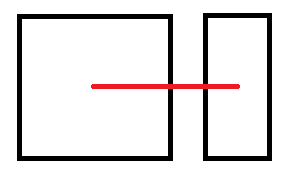
\includegraphics[width=0.5\textwidth]{trailer}
	\caption{Trailer model scheme}
	\label{fig:trailer model}
\end{figure}

The mathematical model of the trailer is represented in \eqref{eq:trailer model}, $u_x$ and $u_y$ are the inputs of the system and represent the speed in the Y and X direction. The angle is represented by $\theta$ , the distance between the driver and the trailer is represented by L. The coordinates of the trailer are represented by $p_x$ and $p_y$.

\begin{equation}
	\begin{cases}
		\dot{p_x} = u_x + L sin \theta \cdot \dot{\theta} \\
		\dot{p_y} = u_y + L cos \theta \cdot \dot{\theta} \\
		\dot{\theta} = \frac{1}{L}(u_ycos \theta - u_x sin \theta)	
	\end{cases}
	\label{eq:trailer model}
\end{equation}

\section{A simple trailer example}
One way of measuring the performance of the library is to compared it to the alternatives. In the following simulation the nmpc-codegen library will be compared to, ForBes zerofrp2 the Matlab implementation of the PANOC algorithm. And to fmincon the internal Matlab solver, using either of the three algorithms interior point, SQP and active set.

\subsection{General performance}
Several NMPC problems can be constructed and solved with nmpc-codegen. Figure~\ref{fig:demos} illustrates the problems used to benchmark nmpc-codegen, they all use the simple trailer model but have different obstacles. The time till convergence is measured, the average time is displayed in table~\ref{tbl:mean time till convergence} in the appendix. While the maximum and minimum time is displayed in the appendix: table~\ref{tbl:min time till convergence} and table~\ref{tbl:max time till convergence}.

The convergence time can be expresses relatively to the convergence time of the nmpc-codegen time as illustrated by \eqref{eq:definition relative time}. These results are displayed in table~\ref{tbl:mean relative time till convergence}. From table~\ref{tbl:mean relative time till convergence} it's clear that nmpc-codegen dominates by a significant margin.

\begin{equation}
	t_{relative} = \frac{t_{algorithm}}{t_{nmpc-codegen}}
	\label{eq:definition relative time}
\end{equation}

\subsection{In-dept analysis of performance}
The in-dept simulation contains four circular obstacles, the trailer will move from the lower left corner to the upper right corner. Each of the algorithms will calculate the optimal path up to the tolerance of $10^{-3}$. The input for one step is then applied to the system equation, and the next state is obtained. The same nmpc problem is solved using the new state as current state  and the new input is applied again.

The state of the trailer will is represented by arrows, the starting point of the arrow is the position of the trailer. The angle of the arrow represents the positional angle of the trailer. The amplitude of the arrow has no meaning. Figure~\ref{fig:simulation result trailer model} contains the results a trailer model simulation. The PANOC algorithm calculated the lowest located path displayed in figure~\ref{fig:solution path trailer example} while all other algorithms like the interior point method of ipopt obtained the upper located path.

Figure~\ref{fig:timings trailer example} shows that the nmpc-codegen library is faster. As nmpc-codegen works completely in C, it has a advantage that has little to do with the algorithm but with the software architecture. Therefore it is advisable to compare PANOC draft and ipopt. PANOC dominates after the first few steps in the simulation. Figure~\ref{fig:timings fmincon Matlab trailer example} shows that this is also the case when comparing PANOC draft with the 3 different fmincon algorithms.

\begin{figure}[H]
	\centering
	\begin{subfigure}[b]{0.45\textwidth}
		\centering
		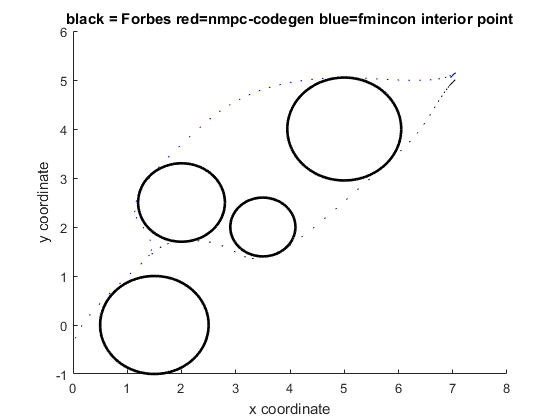
\includegraphics[width=1.2\textwidth]{compare_libs/path}
		\caption{path}
		\label{fig:solution path trailer example}
	\end{subfigure}
	\hfill
	\begin{subfigure}[b]{0.45\textwidth}
		\centering
		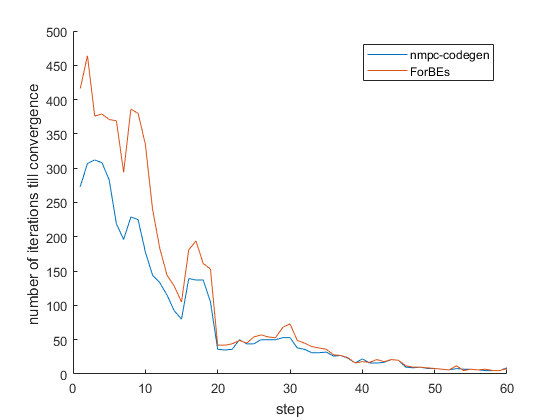
\includegraphics[width=1.2\textwidth]{compare_libs/iterations}
		\caption{iterations}
		\label{fig:iterations trailer example}
	\end{subfigure}
	
	\begin{subfigure}[b]{0.45\textwidth}
		\centering
		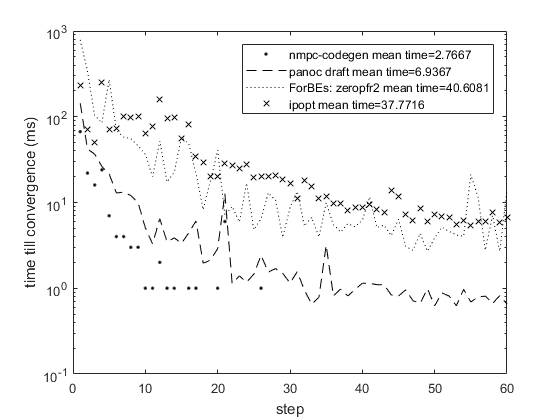
\includegraphics[width=1.2\textwidth]{compare_libs/timings}
		\caption{timings}
		\label{fig:timings trailer example}
	\end{subfigure}
	\hfill
	\begin{subfigure}[b]{0.45\textwidth}
		\centering
		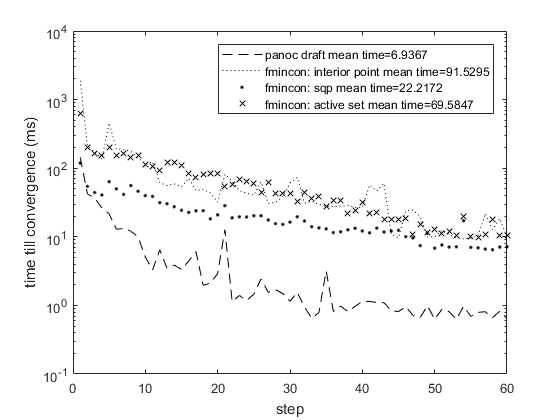
\includegraphics[width=1.2\textwidth]{compare_libs/timings_fmincon}
		\caption{timings}
		\label{fig:timings fmincon Matlab trailer example}
	\end{subfigure}
	\caption{Simulation result trailer model}
	\label{fig:simulation result trailer model}
\end{figure}

The nmpc-codegen library and PANOC draft are using a cautious L-BFGS update which improves the performance of the L-BFGS. This is clear from figure~\ref{fig:iterations trailer example} where not the time till convergence, but the amount of iterations till convergence are illustrated. The nmpc-codegen clearly needs less iterations than  Forbes zerofpr2. As the simulation progresses, less and less iterations are needed to calculate optimal solution. And the L-BFGS doesn't influence the convergence as much, so the two algorithms have about the same amount iterations till convergence. Figure~\ref{fig:timings fmincon Matlab trailer example} show


\section{Quadcopter model}
%TODO: reference source model !!!!!!!!!!!!!!!!!!
The invention of electronic control systems has proven to be especially useful when controlling quadcopters. Because of their complex behavior they are hard to control manually by a pilot. However quadcopters are popular among unmanned aerial vehicles as they can be controlled by a fast digital/analog controller.

\subsection{Mathematical model}
The behavior of a quad copter is described by a set of nonlinear equations as illustrated in \eqref{eq:mathematical model quadcopter}.

\begin{table}[]
	\centering
	\caption{constants used in quadcopter model}
	\label{btl:quadcopter model constants}
	\begin{tabular}{|l|l|l|l|}
		\hline
		Parameter                               & Symbol   & Value             & Unit           \\ \hline
		Mass of the quadcopter                  & m        & 0.5               & kg             \\
		Radius of the quadcopter                & L        & 0.25              & m              \\
		Propeller lift coefficient              & k        & $3 \cdot 10^{-6}$ & $Ns^2$        \\
		Propeller drag coefficient              & b        & $1 \cdot 10^{-7}$ & N m $s^2$      \\
		Acceleration of gravity                 & g        & 9.81              & m/$s^2$        \\
		Air friction coefficient                & $k_d$    & 0.25              & kg/s           \\
		Quadcopter inertia about the $x^b$-axis & $I_{xx}$ & $5 \cdot 10^{-3}$ & kg $m^2$       \\
		Quadcopter inertia about the $y^b$-axis & $I_{yy}$ & $5 \cdot 10^{-3}$ & kg $m^2$       \\
		Quadcopter inertia about the $z^b$-axis & $I_{zz}$ & $1 \cdot 10^{-2}$ & kg $m^2$       \\ 
		Motor constant                          & $c_m$    & $1 \cdot 10^{4}$  & $v^{-2}s^{-2}$ \\
		\hline
	\end{tabular}
\end{table}

\begin{equation}
	\begin{aligned}
		\dot{x} &= v_x \\
		\dot{y} &= v_y \\
		\dot{z} &= v_z \\
		\dot{v_x} &= -\frac{k_d}{m}v_x + \frac{k \cdot c_m}{m}\Big(sin(\gamma)sin(\phi)+cos(\gamma)cos(\phi)sin(\theta)\Big)\Big(u_1 + u_2 + u_3 + u_4\Big) \\
		\dot{v_y} &= -\frac{k_d}{m}v_y + \frac{k \cdot c_m}{m}\Big(cos(\phi)sin(\gamma)sin(\theta)-cos(\gamma)sin(\phi)\Big)\Big(u_1 + u_2 + u_3 + u_4\Big) \\
		\dot{v_z} &= -\frac{k_d}{m}v_y -g + \frac{k \cdot c_m}{m}\Big(cos(\theta)cos(\phi)\Big)\Big(u_1 + u_2 + u_3 + u_4\Big) \\
		\dot{\phi} &= \omega_x + \omega_y\Big( sin(\phi)tan(\theta) \Big) + \omega_z \Big( cos(\phi) tan(\theta) \Big) \\
		\dot{\theta} &= \omega_y cos(\phi) - \omega_z sin(\phi) \\
		\dot{\gamma} &= \frac{sin(\phi)}{cos(\theta)}\omega_y + \frac{cos(\phi)}{cost(\theta)} \omega_z \\
		\dot{\omega_x} &= \frac{Lkc_m}{I_{xx}}\Big( u_1 - u_3 \Big) - \Big( \frac{I_{yy}-I_{zz}}{I_{xx}} \Big) \omega_y \omega_z\\
		\dot{\omega_y} &= \frac{Lkc_m}{I_{yy}}\Big( u_2 - u_4 \Big) - \Big( \frac{I_{zz}-I_{xx}}{I_{yy}} \Big) \omega_x \omega_z\\
		\dot{\omega_z} &= \frac{bc_m}{I_{zz}}\Big( u_1 - u_2 + u_3 - u_4 \Big) - \Big( \frac{I_{xx}-I_{yy}}{I_{zz}} \Big) \omega_x \omega_y\\
	\end{aligned}
	\label{eq:mathematical model quadcopter}
\end{equation}

\subsection{Simulation results}
Figure~\ref{fig:Simulation results with quadcopter} contains a simple simulation with the quad copter model, the path is displayed in figure~\ref{fig:solution path trailer quad}.The quad-copter moves from the star to the circle while avoiding 2 spheres as much as possible. The time to convergence of each step of the simulation is displayed in figure~\ref{fig:timings trailer quad}.

As mentioned at the start of this chapter, the quad copter model is a computational expensive model. This means that the computational cost of solving a system, is more in line with the computational cost of calculating the cost and gradient.

A interior point method solves a system in each iteration. The interior method used from ipopt in this example solves its system directly, which has a computational cost of about $\mathcal{O}(n^3)$ . While PANOC only has to cope additional cost of about $\mathcal{O}(Ln)$ with L as the buffer size.  because the L-BFGS algorithm only uses inner products and vector additions.

This means that the difference between PANOC and ipopt is rather small when using the quad copter model. Which is clearly visible in figure~\ref{fig:timings trailer quad}, where the ipopt line is very near the PANOC draft line.
\begin{figure}[H]
	\centering
	\begin{subfigure}[b]{0.45\textwidth}
		\centering
		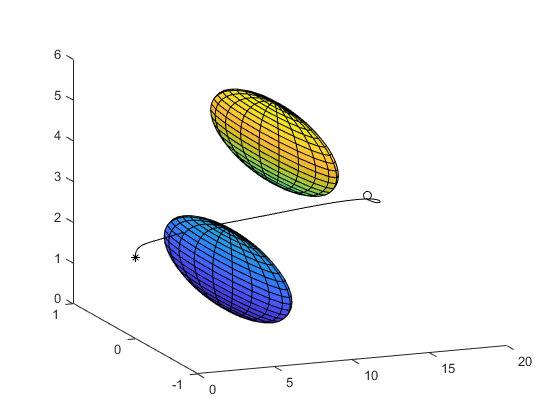
\includegraphics[width=1.2\textwidth]{compare_libs/path_quad}
		\caption{path}
		\label{fig:solution path trailer quad}
	\end{subfigure}
	\hfill
	\begin{subfigure}[b]{0.45\textwidth}
		\centering
		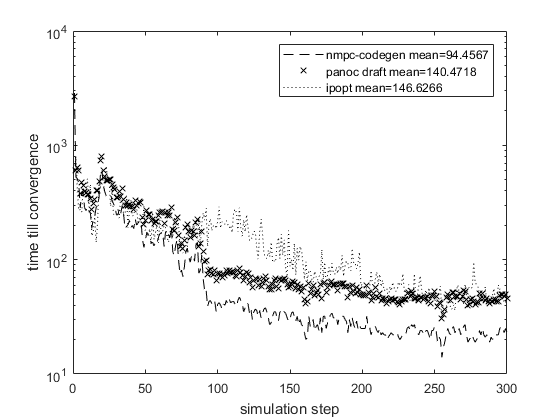
\includegraphics[width=1.2\textwidth]{compare_libs/timings_quad}
		\caption{timings}
		\label{fig:timings trailer quad}
	\end{subfigure}
	\caption{Simulation results with quadcopter}
	\label{fig:Simulation results with quadcopter}
\end{figure}

\section{Influence of noise}
Until now all simulations were executed without any kind of noise. However in reality there is always some kind of state noise. So it is essential to study how PANOC behaves with state noise, more specifically white noise in this case.

The white noise has a maximum amplitude of 0.1 on the x coordinate and the y coordinate. It has a amplitude of 0.05 on the angle $\theta$. The double noise simply doubles the maximum amplitude of the noise. This way the influence of the size of the noise can be studied.

Figure~\ref{fig:Noise simulations with the trailer model} contains the simulation results using PANOC or ipopt as solver. Going from no state noise to a bit of state noise makes a significant difference when solving with PANOC. The interior point method from ipopt, also takes longer to converge when noise is added. However it is much less correlated with the size of the noise, as the interior point method here uses a direct method to solve the system. And doesn't use the initial position to solve its system of equations. However PANOC doesn't seem to slow down a lot when doubling the noise amplitude. Ipopt on the other hand does slows down significantly.

\begin{figure}[H]
	\centering
	\begin{subfigure}[b]{0.45\textwidth}
		\centering
		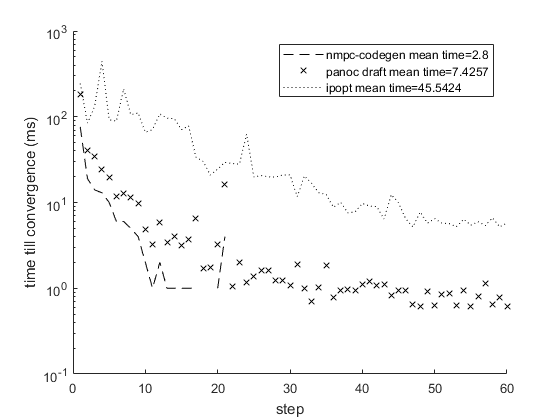
\includegraphics[width=1.2\textwidth]{compare_libs/trailer_without_noise}
		\caption{without noise}
		\label{fig:timings trailer without noise}
	\end{subfigure}
	\hfill
	\begin{subfigure}[b]{0.45\textwidth}
		\centering
		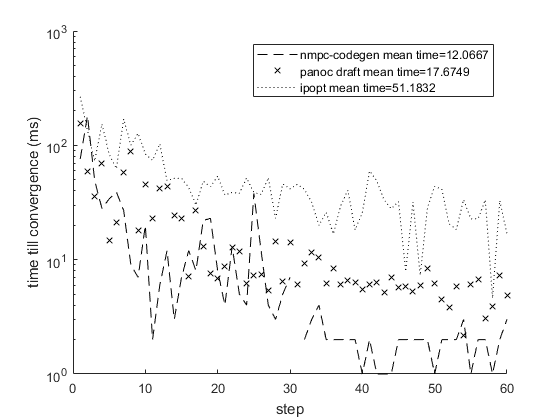
\includegraphics[width=1.2\textwidth]{compare_libs/trailer_with_noise}
		\caption{with noise}
		\label{fig:timings trailer with noise}
	\end{subfigure}
	\begin{subfigure}[b]{0.45\textwidth}
		\centering
		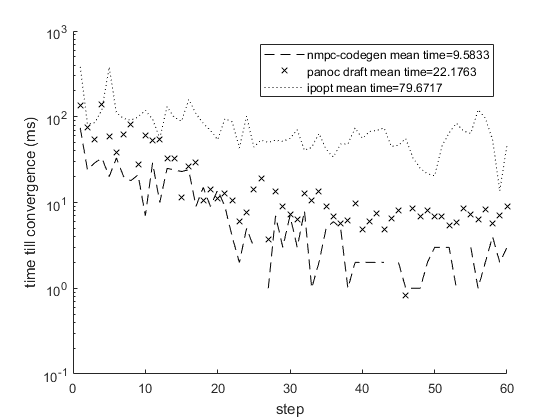
\includegraphics[width=1.2\textwidth]{compare_libs/trailer_with_double_noise}
		\caption{with double noise}
		\label{fig:timings trailer with double noise}
	\end{subfigure}
	\hfill
	\begin{subfigure}[b]{0.45\textwidth}
		\centering
		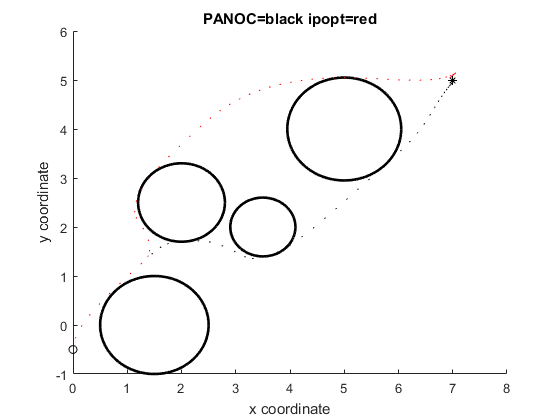
\includegraphics[width=1.2\textwidth]{compare_libs/path_without_noise}
		\caption{path without noise}
		\label{fig:path noise simulations}
	\end{subfigure}
	\caption{Noise simulations with the trailer model}
	\label{fig:Noise simulations with the trailer model}
\end{figure}

\begin{table}[H]
	\centering
	\begin{tabular}{|l|c|c|c|c|}
		\hline
		&\textbf{no noise}&\textbf{with noise}&\textbf{double noise}\\\hline
		\textbf{nmpc-codegen}&3 ms&12 ms&10 ms \\\hline
		\textbf{draft PANOC}&8 ms&18 ms&22 ms \\\hline
		\textbf{OPTI:ipopt}&45 ms&51 ms&80 ms \\\hline
	\end{tabular}
	\caption{average till convergence in milliseconds}
	\label{tbl:average till convergence noise}
\end{table}

\section{Problem with local minimum}
One problem with the approach discussed in this chapter, is visible in the third demo. The results of the third demo are illustrated in figure~\ref{fig:demo: local minimum problem}, the trailer drives through the obstacle which might be impossible in reality. In reality the trailer might crash into the obstacle, and get stuck. Of course it is possible to increase the weight on the obstacle, this will make the problem harder. As the condition will get worse, and the solution will be about the same. The trainer will get stuck against the obstacle. PANOC is stuck inside a local minimum.

\begin{figure}[H]
	\centering
	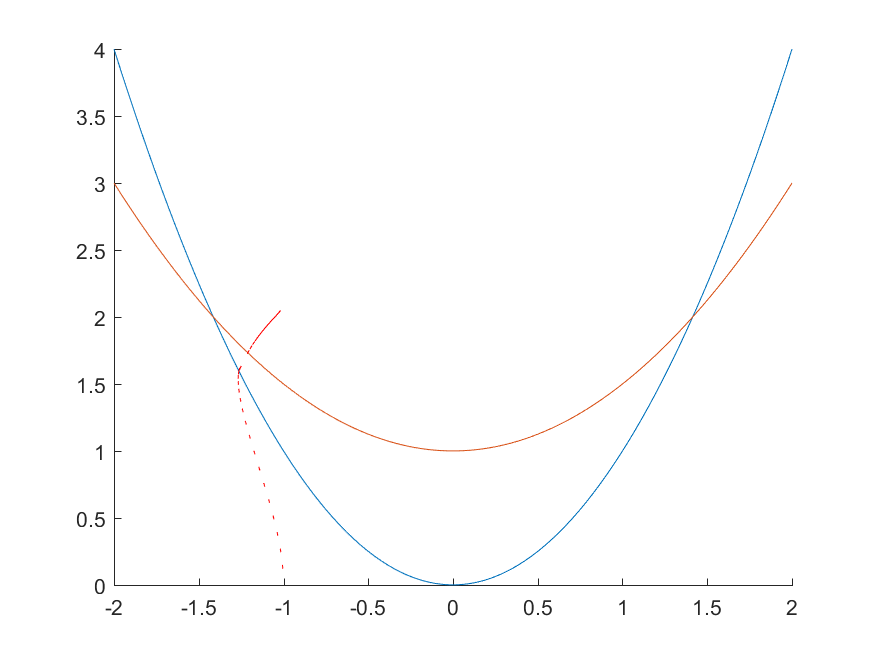
\includegraphics[width=0.5\textwidth]{demos/demo3}
	\caption{Local minimum problem}
	\label{fig:demo: local minimum problem}
\end{figure}

\section{Conclusion}

The simulations clearly indicate that a great speed up his gained by implementing the PANOC algorithm in C. As the algorithm doesn't require a lot of memory it can be run efficiently on small embedded devices. PANOC behaves very well when noise is introduced. The performance of PANOC is very good compared to ipopt if the models are simple. However as the models get more complex, PANOC loses its speed edge over ipopt.